\subsection{Systematic uncertainties}
\label{sec:systematics}


The inputs to the combination all have their individual systematic uncertainties, summarized in Section~\ref{sec:inputs}.
% 
The systematic uncertainties are implemented in the extended likelihood as nuisance parameters and are profiled in the fit.
% 
For the purpose of the combination, it is important to associate the correct correlations between systematic uncertainties of the individual analyses, and to associate an additional uncertainty due to unfolding to full phase space rather than a fiducial one.
% 
Among the decay channels, correlations are taken into account for the systematic uncertainties in the jet energy scale and resolution, and the integrated luminosity.


As explained in more detail in Sections~\ref{hgg,hzz}, the individual $\hgg$ and $\hzz$ analyses from Refs.~\cite{Sirunyan:2018kta,Sirunyan:2017exp} are extrapolated to their respective fiducial phase spaces.
% 
A fiducial phase space is a conveniently chosen phase space which avoids poorly understood regions, such as the very-forward (high $\eta$) region, which in turn reduces the systematic uncertainties related to the extrapolation.
% 
While fiducial phase spaces are useful in the case of a single-channel analysis, there is no clear way of combining results obtained in different fiducial phase spaces.
% 
In order to combine multiple channels, the data have to be unfolded to a common phase space, which is commonly chosen to be the full phase space.
% 
The main systematic uncertainties associated with this extrapolation concern uncertainties in the detector acceptances and, if not profiled in the fit, the overall normalization of Higgs boson production modes.


% ____________________________________________________________________________
% Acceptances

The most pressing concern when unfolding to the full phase space, is the uncertainty on the detector acceptance, especially in the poorly understood regions of the detector.
% 
The acceptances are calculated using a Monte Carlo simulation.
% 
The corresponding uncertainties are calculated by varying the renormalization and factorization scales $\mu_R$ and $\mu_F$ in the simulation, and applying the so-called \emph{envelop method} on the resulting acceptances: The acceptance uncertainty per bin is given by the minimum and maximum variations.
% 
The scales $\mu_R$ and $\mu_F$ are allowed to vary independently, under the condition that $\frac{1}{2} < \frac{\mu_R}{\mu_F} < 2$.
% 
The effect of the acceptance uncertainties on the $\pth$ distribution is shown in Table~\ref{tab:accuncertainties}, where the acceptance uncertainties are added in quadrature to the expected systematic uncertainties of the combined $\pth$ distribution.
% 
On solely the systematic uncertainty, the effect of the acceptance uncertainties is expected to be non-negligible in only two bins, $[45,80)$ and $[350,600)$; on the total uncertainty the effect is negligible throughout.
% 
Given the negligibly small impact, the acceptance uncertainties are neglected for the final results in Section~\ref{diffresults}.

\begin{table}[h!]
\footnotesize
\caption{
    Acceptance uncertainties and the relative change they manifest when added in quadrature to the uncertainties of the $\pt$ combination.
    }
\label{tab:accuncertainties}
\begin{center}
\setlength\tabcolsep{3pt}
\begin{tabular}{lccccccccc}
Bins                      & $[0,15)$ & $[15,30)$ & $[30,45)$ & $[45,80)$ & $[80,120)$ & $[120,200)$ & $[200,350)$ & $[350,600)$ & $[600,\infty)$  \\
\hline
Acc. uncertainties        & 0.6\%   & 1.3\%    & 2.8\%    & 5.7\%    & 1.0\%     & 1.7\%      & 4.1\%      & 10.2\%     & 28.8\%  \\
Rel. change in syst. unc. & 0.3\%   & 0.7\%    & 4.1\%    & 19.7\%   & 0.3\%     & 1.8\%      & 2.0\%      & 7.6\%      & 1.0\%   \\
Rel. change in tot. unc.  & 0.0\%   & 0.1\%    & 0.3\%    & 1.2\%    & 0.0\%     & 0.1\%      & 0.2\%      & 0.3\%      & 0.2\%   \\
\end{tabular}
\end{center}
\end{table}


% ____________________________________________________________________________
% xH normalization uncertainty

When certain production modes are assumed to be at their SM values in a fit, the fit must include a systematic uncertainty related to the normalization of these processes.
% 
For most differential cross sections all production modes are fitted simultaneously, and thus no further systematic uncertainty is needed.
% 
In the case of the $\pth$ spectrum of only Higgs bosons produced via gluon fusion, the uncertainty on the normalization of the other modeled production modes is included as a nuisance parameter.
% 
The uncertainties per production mode are shown in Table~\ref{tab:xhunc}.
% 
The uncertainty on the normalization of non-$\ggh$ production modes is calculated to be $2.1\%$.
% 
It is implemented as a constant uncertainty throughout the $\pth$ spectrum in the fits that assume a SM normalization for non-$\ggh$ production modes.


\begin{table}[h!]
\footnotesize
\caption{
    Uncertainties on the overall normalizations of Higgs production modes other than $\ggh$, taken from Ref.~\cite{deFlorian:2016spz}.
    % 
    The overall normalization uncertainty of all production modes other than $\ggh$ combined is found to be $2.1\%$
    }
\label{tab:xhunc}
\begin{center}
\begin{tabular}{llcccl}
Production mode  &  $\sigma$ (pb)  &  $\Delta$Scale ($\%$)  &  $\Delta$PDF ($\%$)  &  $\Delta\alpha_s$ ($\%$)  &  Total (pb) \\
\hline
$\vbf$                               & $3.78$                & $0.35\%$     & $2.1\%$      & $0.05\%$            & $8.05 \cdot 10^{-2}$ \\
$\wboson\hboson$                     & $1.37$                & $0.6\%$      & $1.7\%$      & $0.9\%$             & $2.76 \cdot 10^{-2}$ \\
$\zboson\hboson$                     & $8.82 \cdot 10^{-1}$  & $3.4\%$      & $1.3\%$      & $0.9\%$             & $3.31 \cdot 10^{-2}$ \\
$\tth$                               & $5.06 \cdot 10^{-1}$  & $7.5\%$      & $3.0\%$      & $2.0\%$             & $4.21 \cdot 10^{-2}$ \\
$\bbh$                               & $4.86 \cdot 10^{-1}$  & $22.0\%$     & $0.0\%$      & $0.0\%$             & $1.07 \cdot 10^{-1}$ \\
$\tquark\hboson (\text{t-channel})$  & $7.43 \cdot 10^{-2}$  & $10.6\%$     & $3.5\%$      & $1.2\%$             & $8.34 \cdot 10^{-3}$ \\
$\tquark\hboson (\text{s-channel})$  & $2.87 \cdot 10^{-3}$  & $2.1\%$      & $2.2\%$      & $0.2\%$             & $8.76 \cdot 10^{-5}$ \\
\hline
Total                                & $7.10$                &              &              &                     & $0.15$ ($2.1\%$) \\
\end{tabular}
\end{center}
\end{table}


The total systematic uncertainty, with and without the inclusion of an additional uncertainty due to the normalization on the non-$\ggh$ production modes, is shown in Table~\ref{tab:effect-of-xhunc}.
% 
While the systematic uncertainty increases slightly, the overall effect is small.

\begin{table}[h!]
\footnotesize
\caption{
    Systematic uncertainty of the $\pth$ spectrum, where the Higgs boson is produced exclusively via $\ggh$, with and without an additional systematic uncertainty related to the normalization of the non-$\ggh$ production modes.
    }
\label{tab:effect-of-xhunc}
\begin{center}
\setlength\tabcolsep{3pt}
\begin{tabular}{lccccccccc}
$\pth$  (\GeV)  & $0-15$      & $15-30$     & $30-45$     & $45-80$     & $80-120$    & $120-200$   & $200-350$   & $350-600$    & $600-850$    \\
\hline 
$\Delta_\text{syst}$ w/o non-$\ggh$ norm. unc. & $6.97\%$  & $6.35\%$  & $7.41\%$  & $8.16\%$  & $8.98\%$  & $10.44\%$ & $11.16\%$ & $23.43\%$  & $117.16\%$ \\
$\Delta_\text{syst}$ w/ non-$\ggh$ norm. unc.  & $6.97\%$  & $6.38\%$  & $7.41\%$  & $8.17\%$  & $9.01\%$  & $10.52\%$ & $11.26\%$ & $23.57\%$  & $117.17\%$
\end{tabular}
\end{center}
\end{table}

% The $\pth$ spectrum via $\ggh$ is shown in Fig.~\ref{fig:xH_uncertainty_impact} with and without the uncertainty on the other production modes included.
% % 
% The uncertainty manifests itself visibly in the systematic uncertainty, although the result is not significantly altered.


% \begin{figure}[hbtp]
%   \begin{center}
%     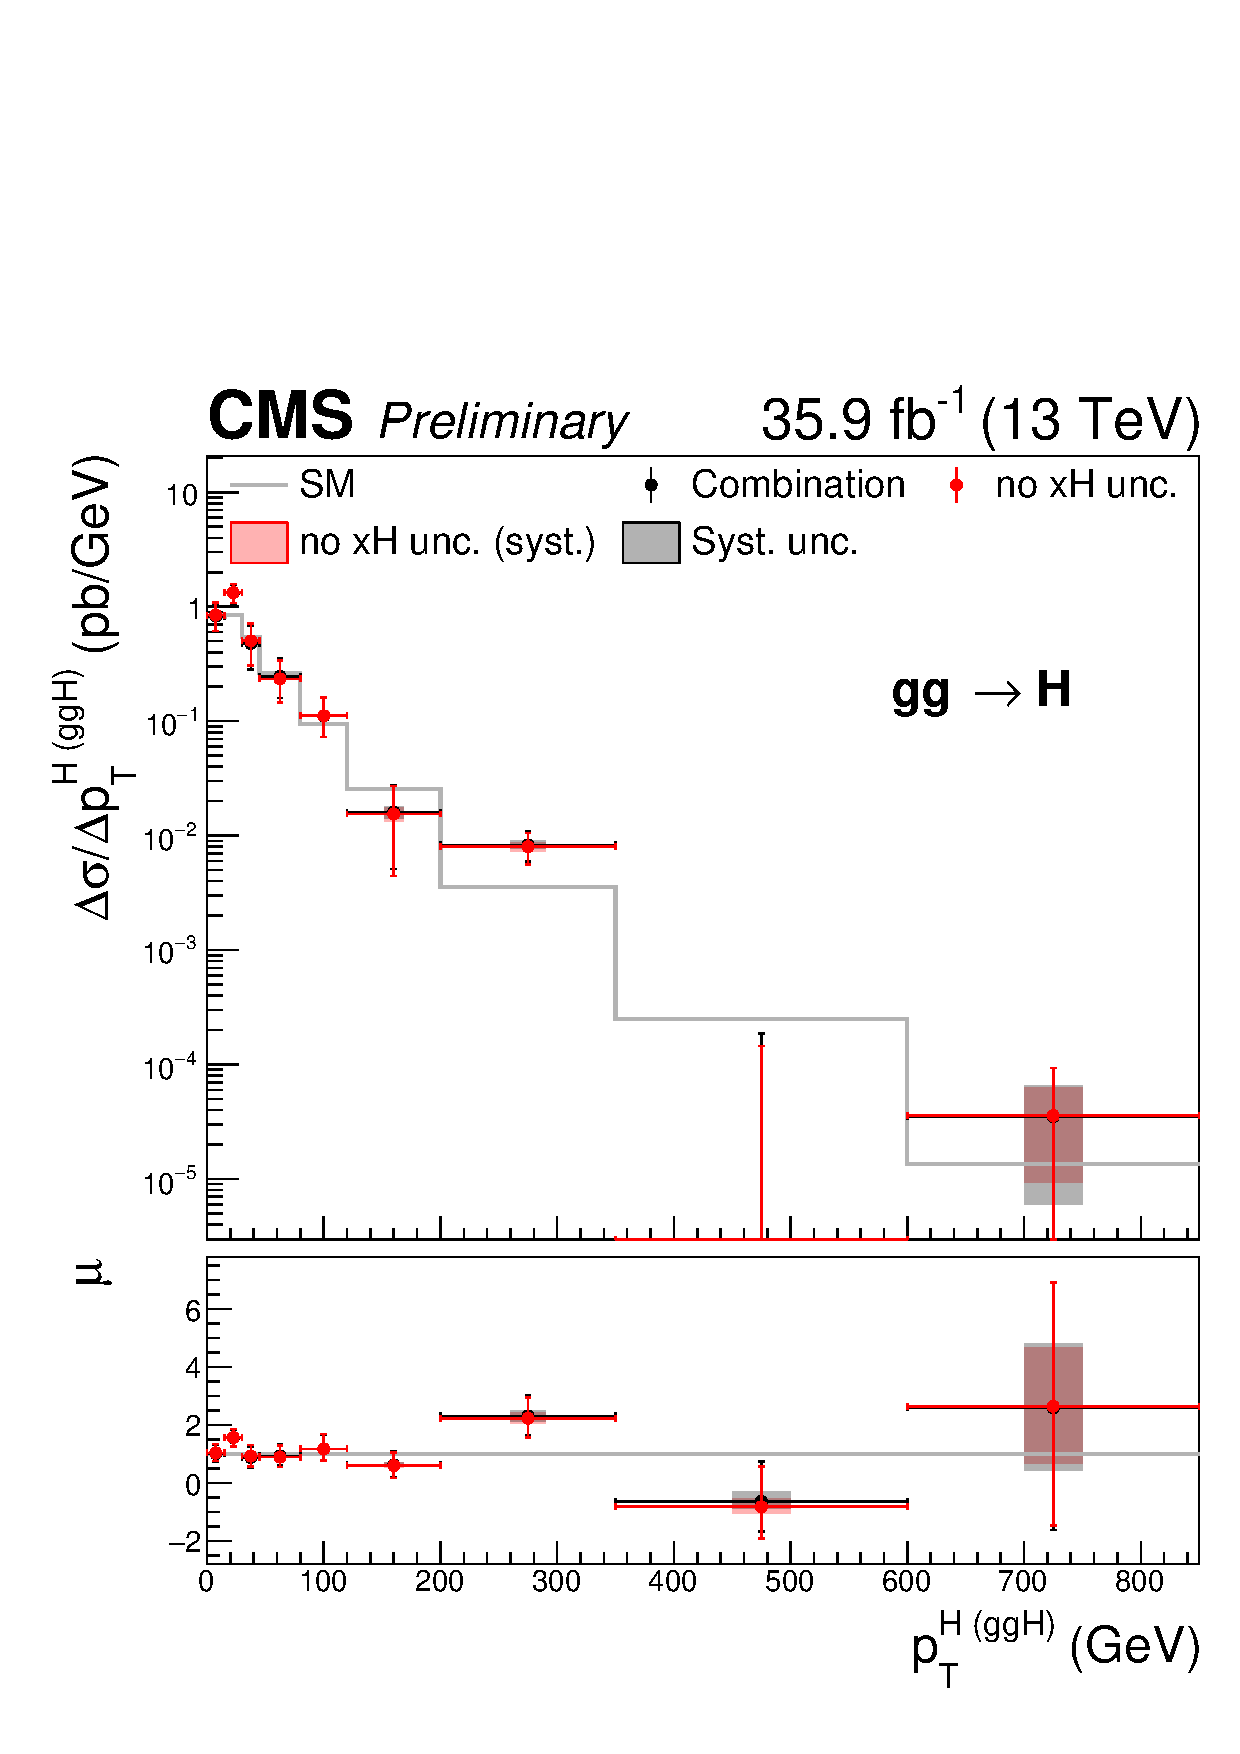
\includegraphics[width=\halflinewidth]{img/differentials/comparison_including_xH_unc.pdf}
%     % 
%     \caption{
%         Combination of $\pt^\text{ggh}$, using the $\hgg$, $\hzz$ and $\hbb$ decay channels. 
%         % 
%         \tk{Edit caption, and repeat this on the Asimov!}
%         }
%     \label{fig:xH_uncertainty_impact}
%   \end{center}
% \end{figure}

